\documentclass[../../../main.tex]{subfiles}

\begin{document}

The advanced STEM courses I have taught thus far at Whittier College are now introduced, with connections to departmental goals and learning focuses listed in Sec. \ref{sec:methods}.
\\
\vspace{0.25cm}
\textbf{\textit{Computer Logic and Digital Circuit Design (PHYS306/COSC330)}}. Computer Logic and Digital Circuit Design is cross-listed as PHYS306/COSC330.  My first goal for the students was to impart my advanced learning focus of \textbf{strength in all phases of science}, and \textbf{to satisfy departmental goals 4-7}.  This is a 300-level course that satisfies core requirements in the following majors: Physics, ICS/Physics, ICS/Economics, 3-2 Engineering/Math, 3-2 Engineering/Computer Science.  Such a broad course that serves a wide variety of students should touch on at least the following sub-topics:

\begin{enumerate}
\item Binary mathematics, non-decimal base systems, and boolean logic
\item Basic digital components, clocks and gates
\item Implementation of boolean algebra with digital components
\item Complex digital components
\item Creation of digital circuits and projects
\item Analysis of digital data, analogue-to-digital and digital-to-analogue conversion
\end{enumerate}

Covering the topics above with challenging content is how I reach my first advanced course learning focus of \textit{mental discipline.}  Additionally, any good digital design course must evenly cover the following phases of the field: \textit{mathematics, computer programming and modeling, hardware design and testing, and digital data analysis} (strength in all phases of science)\footnote{An example syllabus is in the supporting material.}.  The final learning focus is \textit{communication}, and we reach this learning goal through final group-projects.  The students submit a project proposal before beginning work, and we polish presentations in office hours in advance of the final presentation.
\\
\vspace{0.25cm}
Half of each class period is dedicated to making progress on the digital design labs using the PYNQ-Z1 system-on-a-chip (SoC).  To set up a system for the student pair, I install a Linux operating system on a laptop, and use it to download an operating system for the SoC.  The PYNQ-Z1 is called a SoC because it has both programmable logic firmware (PL) and a processing system (PS) like a small computer.  The default operating system for PYNQ-Z1 contains basic examples that show the students how to use the digital components of the SoC.  By the end of the course, the students are writing code in Python3 that literally creates digital circuits inside the SoC.  They use the boards to learn, and to build projects.  Diagrams of the system are shown in Fig. \ref{fig:pynq}.
\\
\vspace{0.25cm}
Using the boards, I provide a bridge to another course, digital signal processing (DSP, see below), by leading the students to a special activity.  The students capture analogue voltage signals from an external source, digitize it using the SoC, and graph it using Python3.  This lab activity is a model for how sensors work, and the starting point for DSP.  The final projects for this course were stiffled by the remote learning situation in Spring 2020.  My hope is that the students will design sensors, timing-based systems like traffic-light controllers, and video processing.  Personally, I have processed HDMI video and remote audio with the PYNQ-Z1 SoC.  Though these projects might be more challenging for the students, I know one or two groups will give these a shot.
\\
\vspace{0.25cm}
The other half of COSC330/PHYS306 class periods are spent learning number systems like binary and hexidecimal, boolean logic and boolean algebra, and logic functions.  When woven together, these concepts give the students a basic understanding of how embedded digital systems function.  Imagine a system designed to fill bottles with pills via a conveyor belt and valve.  Imagine how the number of pills would be counted in binary, and how that result would control both the conveyor and the valve.  The students devise solutions to situations like the pill bottle one, using conceptual tools from lecture period.  We also cover how these tools have applications in business.  One main example is how to simplify a logic function, and how that technique can simplify a business workflow.
\\
\vspace{0.25cm}

\begin{figure}
\centering
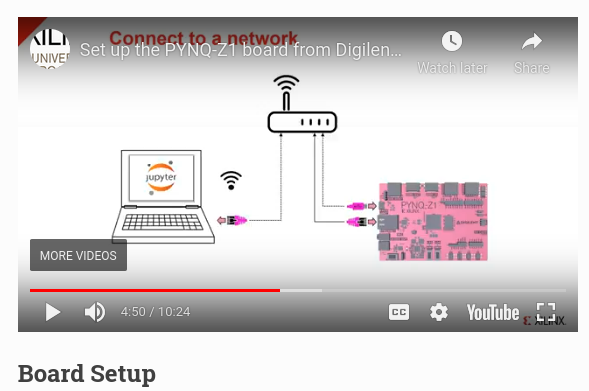
\includegraphics[width=0.4\textwidth]{figures/pynq1.png}
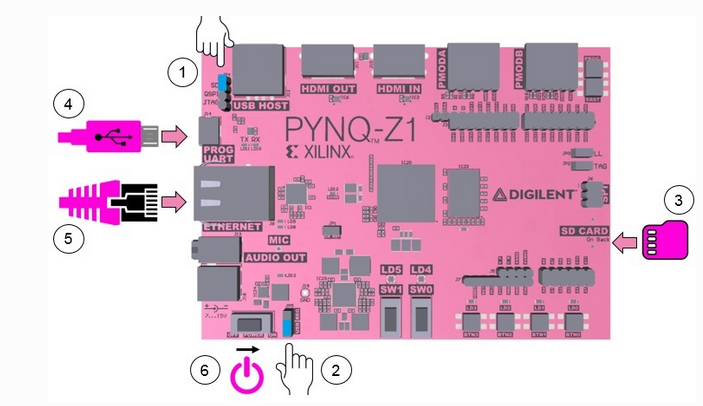
\includegraphics[width=0.4\textwidth]{figures/pynq2.png}
\caption{\label{fig:pynq} (Left) A setup video explaining how to connect a laptop to the PYNQ-Z1 system. (Right) A diagram of the PYNQ-Z1 system-on-a-chip (SoC).  The board has a microprocessor, programmable logic, ethernet and USB connections, and a small operating system installed on an SD card.}
\end{figure}

\textbf{\textit{Digital Signal Processing (COSC390)}}.  Digital Signal Processing (DSP) was listed as COSC390 in January term of 2019.  COSC390 is a 300-level integrated computer science course that satisfies core requirements in the following majors: Physics, ICS/Physics, ICS/Economics, 3-2 Engineering/Math, 3-2 Engineering/Computer Science.  I also keep in mind \textbf{Physics Department goals 4-7} when implementing this course.
\\
\vspace{0.25cm}
DSP encompasses the myriad of ways we capture, process, and filter analogue signals like audio signals, medical sensors on the heart and brain, and images.  DSP gives students vital skills such as loading, cleaning, manipulating, and graphing data.  DSP is used by a wide variety of students in fields beyond engineering.  For example, at Rio Hondo Community College, students apply DSP in Sound Design \cite{rio_hondo}.  Our students also practice a vital skill in DSP: Fourier analysis.  This technique allows a student rearrange data comprised of \textit{time-dependent} signals into \textit{frequency-dependent} signals, like tuning a radio to the right frequency.  One economics student, for example, was able to find periodic trends in the stock market using this technique.
\\
\vspace{0.25cm}
When I last taught DSP, the students were a diverse group.  Their majors ranged from business, economics, WSP, ICS/Math, and Physics.  My students were 60\% people of color, and ranged from sophomores to seniors.  The minimum number of students for a course was five, so I actively recruited students.  I got permission to promote my new course in person in pre-requisite courses like COSC120 and MATH141.  The students for whom January term was not booked signed up excitedly.  My diverse group of students had great success, and learned key career skills.  Finally, they did not pay a cent for books or software because it was 100\% open access.  I will be teaching DSP for the second time this coming January term, and I plan to expand my recruitment to majors like Art and Digital Design, and music.  I mention diversity and inclusion here only because one professor emailed me with a question about inclusion and DSP. 
\\
\vspace{0.25cm}
To reach my first advanced learning focus of \textit{mental discipline}, my students engaged with modules requiring analytic and creative thinking.  Because this was a January term course, we met for three hours each morning for three weeks.  Homework sets were assigned each day, and kept \textit{short}, but challenging.  This is the first time I tried such a style, but the students found it refreshing and efficient.  The style ensured that the problems I assigned came straight from the lecture of that day (or occasionally one day prior).  Another benefit of the cadence was that if a student was struggling, I could identify and help them very quickly.
\\
\vspace{0.25cm}
The second learning focus for advanced courses is \textit{strength in all phases of science.}  COSC390 follows COSC330/PHYS306 conceptually.  One can think of COSC330/PHYS306 as learning the building blocks of digital components.  Some of those components help create scientific instruments that sample and digitize analog data.  Digital Signal Processing (DSP) is the subject of what follows \textit{after} the sampling and digitization (i.e. the next phase).  I broadened the content to sub-topics like financial data analysis, which may be analyzed with DSP.  One of the student-designed projects in COSC390 was an analysis of Federal Reserve interest rate data over many decades using DSP.  Other presentations included image processing within the context of criminal justice (facial identification), and audio capture and processing of the guitar music of a student.  For the projects, the students engaged more in the final two phases I identified in Sec. \ref{sec:methods}, whereas they engaged more in the first two in COSC330/PHYS306.
\\
\vspace{0.25cm}
\textbf{\textit{Electromagnetic Theory (PHYS330)}}.  Electromagnetic theory is a course taught in every department of physics.  It is an advanced theoretical physics course utilized by 3-2 engineering, chemistry, and physics students.  It builds upon vector calculus (MATH241) and PHYS180, and vector calculus is built from single-variable calculus (MATH141 and MATH142).  I taught this course under the module system for the first time in Fall 2020.  I utilized my standard fare of warm-up exercises, TT modules, and PER.  However, the students in this course are mostly juniors and seniors whom we have already engaged in pre-requisite courses.  Thus, they prefer more TT modules and fewer PER modules.
\\
\vspace{0.25cm}
The first learning focus is \textit{mental discipline}, so I begin the course with a rigorous review of vector calculus, augmented with custom videos (See Fig. \ref{fig:video}).  With the module system, students had to develop final project plans early in the course before they had seen most of the material.  We had to strike a balance between going too fast (in order to introduce them to enough material to create final projects), and going too slow (to prevent students from getting lost).  We use the ubiquitous textbook for this course entitled \textit{Introduction to Electrodynamics, 3rd ed.} by David Griffiths.  When I was in college, we used the 2nd edition and spent one 14-week semester covering most of the book.  Other institutions spend two full semesters covering the whole book\footnote{I took this course in 2004 at Yale University, whereas a friend I met at Los Alamos National Laboratory told me her course in the same year was half the pace, for two semesters, at Northern Arizona University.}.  My task was to cover the first half of the book in just seven weeks\footnote{For more information, see my syllabus in supporting material.}.
\\
\vspace{0.25cm}
\begin{figure}
\centering
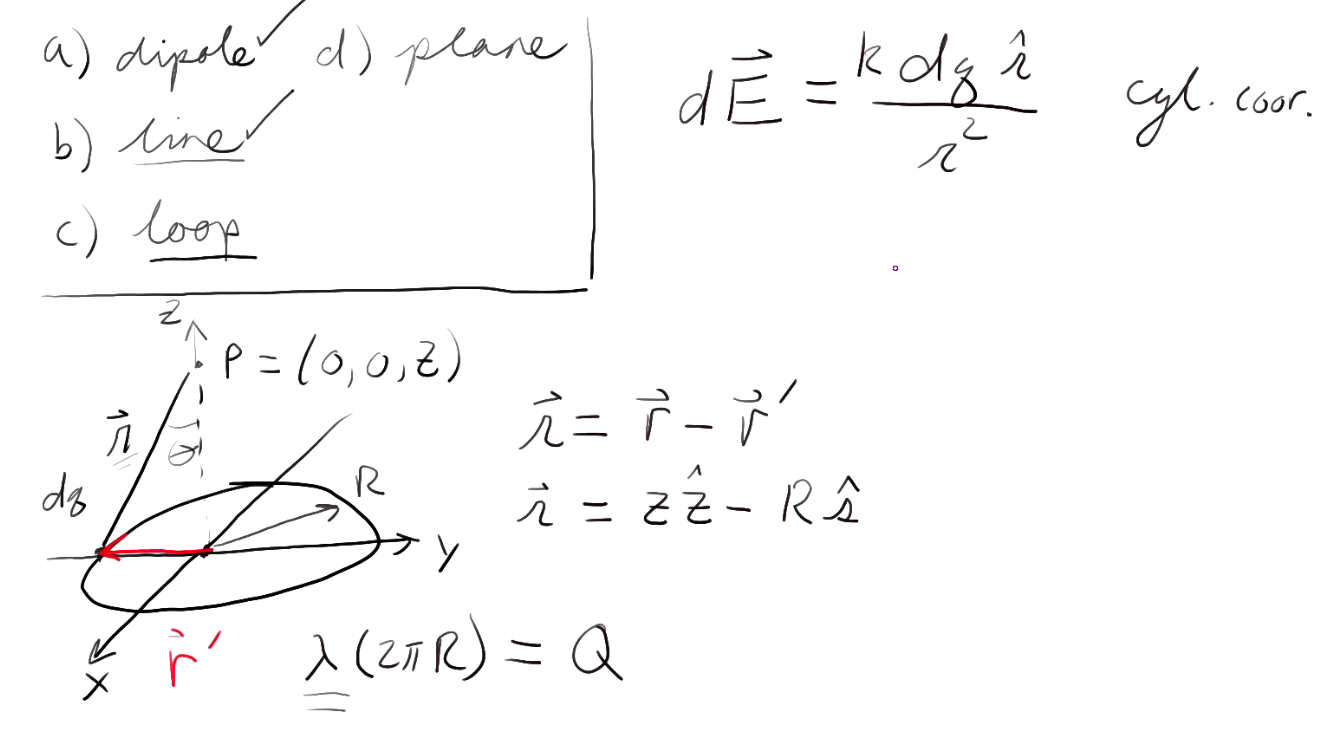
\includegraphics[width=0.6\textwidth]{figures/video_330.png}
\caption{\label{fig:video} A screenshot of a video I produced for my students to help refresh their memories regarding electromagnetism and calculus.}
\end{figure}

The second and third learning focuses are \textit{strength in all phases of science,} and \textit{communication.}  PHYS330 is one of our upper-division electives that is centered on abstract problem-solving and numerical prediction/modeling, so there is rarely any focus on the third and fourth phases.  Although most of our time is spent on building theoretical ideas that the students will use in engineering or see once more in graduate school, I did include some demonstrations of modern electromagnetism: CEM.  CEM stands for computational electromagnetism, and I discuss it further in Sec. \ref{sec:scholarship}.  I coached some students through some CEM calculations for their final projects, while others demonstrated how to solve particularly challenging homework problems for the class.  Final projects included topics like electromagnetic radiation, the intersection of quantum mechanics and electromagnetism, and the electric fields of interesting shapes of electric charge.  Most students took the course to apply towards their major, and reported that they learned the material well, if only for seven weeks.

\end{document}
